\section{Experimental Results}
\ifCLASSOPTIONonecolumn\begin{figure*}[t]
\centering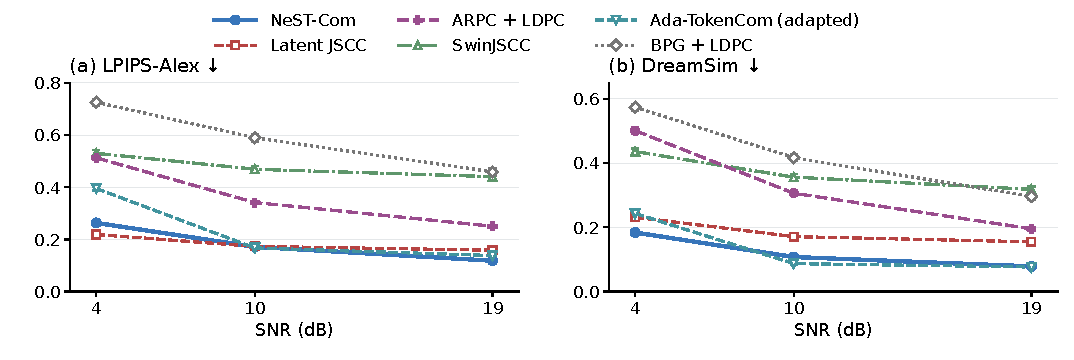
\includegraphics[width=\textwidth]{figure2.pdf}
\caption{Source-referenced perceptual distances on common500 at $N=1024$. Points and error bars are equal-source means and pointwise 95\% source-bootstrap intervals after averaging three channel outcomes per source. Lower LPIPS-Alex and DreamSim are favorable. Ada denotes the predicted-class, fixed-frame adaptation.}
\label{fig:performance}
\end{figure*}
\fi
\subsection{Experimental Setup}
We use common500 ImageNet validation images~\cite{imagenet}, a disjoint cal1000 set, and Kodak24~\cite{kodak}, with fixed $256\times256$ preprocessing. ImageNet-calibrated policies remain fixed on Kodak. The six-system main study uses $N=1024$; NeST, WHOLE, and Ada also use $N=512$, each independently calibrated at 4/10/19~dB.

Our convolutional Latent JSCC maps tokenizer latents to symbols and shares $\Dc$, using MSE, LPIPS, and latent-consistency losses. It and SwinJSCC~\cite{swinjscc}, adapted to $256\times256$ and $N{=}1024$, use the same 20\,000 training images and final 100k/200k-update checkpoints. Digital baselines are adaptive BPG~\cite{bpg} + LDPC, ARPC~\cite{arpc} + LDPC with paid captions, and Ada-TokenCom~\cite{adatokencom} adapted to the fixed single-frame budget. Ada retains LlamaGen-L/VQ16 and prefix arithmetic coding, with a fixed ConvNeXt predicting a paid 10-bit class. Its sampled tail uses CFG=4, $T=1$, top-$k=2000$, and top-$p=1$. Supplement~S1.2 details the six adaptations and their calibration objectives and populations. NeST, WHOLE, and Ada select QPSK rate 2/3, 16-QAM rate 2/3, and 64-QAM rate 5/6 at 4/10/19~dB, respectively, at both budgets; S1.1 lists their targets.

We evaluate source-referenced LPIPS-Alex~\cite{lpips} and DreamSim~\cite{dreamsim}, pixel fidelity by PSNR, and image-feature similarity by CLIP ViT-L/14 cosine (CLIP-I)~\cite{clip}. Frozen FP32 preprocessing uses $224\times224$ bicubic-antialias inputs for DreamSim/CLIP. Three channel outcomes per image, including gray failures, are averaged before equal-source means and direct source-paired 95\% bootstrap intervals (10\,000 resamples). Controls use a fixed 100-image subset. DINOv2 selects generative transmission policies; it is related to feature-based evaluation, rather than an independent perceptual validation.

\ifCLASSOPTIONonecolumn\else\begin{figure*}[t]
\centering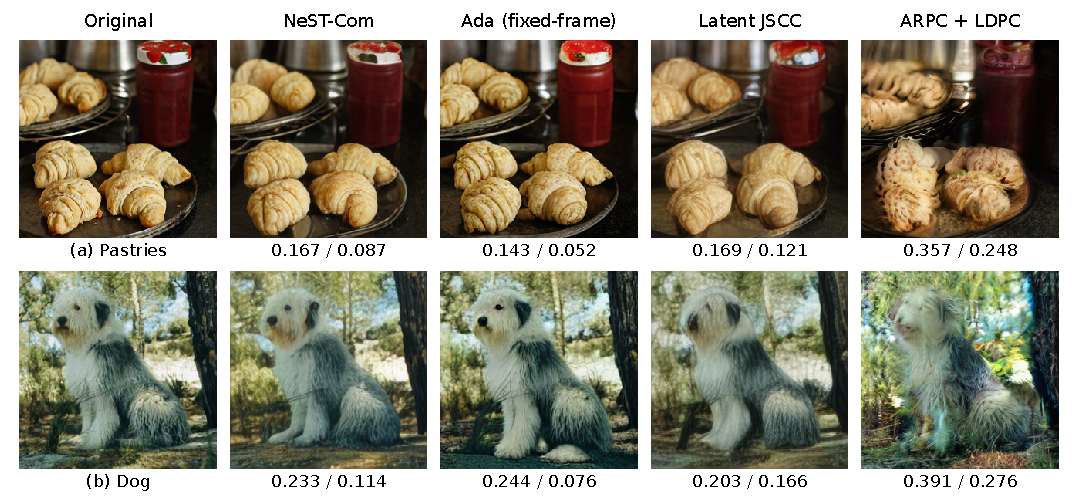
\includegraphics[width=\textwidth]{figure3.pdf}
\caption{Qualitative reconstructions of two development examples at $N=1024$ and 10~dB. Values denote LPIPS-Alex$\downarrow$ / DreamSim$\downarrow$. Ada denotes the fixed-frame adaptation.}
\label{fig:qualitative}
\end{figure*}
\fi
\subsection{Effect of Within-Scale Endpoints}
\begin{table}[t]
\caption{Within-scale endpoint and receiver evidence. (A) Main family-specific policies, PARTIAL minus WHOLE. (B) Fixed 100-source model/MCS/maximum-endpoint control. (C) Ordered interventions on the same 100 sources and actual prefixes. Brackets give source-paired 95\% CIs.}
\label{tab:internal}
\centering\footnotesize
\setlength{\tabcolsep}{2.5pt}
\begin{tabular}{ccc}
\toprule
\multicolumn{3}{l}{(A) Main policies at $N=1024$} \\
SNR & Util. W$\to$P (\%) & $\Delta$LPIPS [95\% CI] \\
\midrule
\multicolumn{3}{l}{common500} \\
4 & 73.81 $\to$ 93.08 & $-0.0246\;[-0.0262,-0.0230]$ \\
10 & 77.70 $\to$ 95.21 & $-0.0273\;[-0.0296,-0.0249]$ \\
19 & 85.24 $\to$ 94.73 & $-0.0052\;[-0.0056,-0.0048]$ \\
\multicolumn{3}{l}{Kodak24} \\
4 & 75.69 $\to$ 93.43 & $-0.0189\;[-0.0247,-0.0130]$ \\
10 & 78.11 $\to$ 94.99 & $-0.0267\;[-0.0370,-0.0167]$ \\
19 & 85.69 $\to$ 93.71 & $-0.0038\;[-0.0056,-0.0022]$ \\
\midrule
\multicolumn{3}{l}{(B) Fixed-granularity diagnostic, 10 dB} \\
Grid (candidates) & Utilization (\%) & LPIPS \\
Whole (7) & 78.15 & 0.2018 \\
Half (13) & 89.21 & 0.1838 \\
Quarter (25) & 95.38 & 0.1752 \\
Eighth (49) & 97.39 & 0.1729 \\
\midrule
\multicolumn{3}{l}{(C) Receiver interventions: $\Delta$LPIPS [95\% CI]} \\
SNR & B0$-$A0 & C0$-$B0 \\
10 & $-0.0100$ & $-0.0166$ \\
 & $[-0.0120,-0.0080]$ & $[-0.0205,-0.0129]$ \\
19 & $-0.0051$ & $+0.0000$ \\
 & $[-0.0060,-0.0043]$ & $[0.0000,0.0000]$ \\
\bottomrule
\end{tabular}
\par\smallskip\parbox{\columnwidth}{\footnotesize Boundary tokens: A0, unused; B0, residual correction only; C0, residual correction and conditioning update. All three use the received complete coarse scales.}
\end{table}

Table~\ref{tab:internal}(A) compares WHOLE/PARTIAL with shared tokenizer, prior, entropy coder, and $\Dc$. Separate family calibration selects the same MCS at each SNR. At $N=1024$, 10~dB, utilization rises from 77.70\% to 95.21\%, retaining more source tokens. Mean LPIPS falls from 0.198718 to 0.171465 and DreamSim from 0.131728 to 0.107680: relative metric reductions of 13.7\% and 18.3\%. Their paired differences are $-0.0273\,[-0.0296,-0.0249]$ and $-0.0240\,[-0.0270,-0.0212]$. LPIPS and DreamSim improve at all six common500 budget/SNR points, with intervals excluding zero (Supplement~S2.4). The N1024 PSNR gains are 0.32--0.70~dB. Kodak LPIPS also improves at all three SNRs; its 19~dB DreamSim interval includes zero.

Block~B fixes 100 sources, the model, MCS, maximum endpoint, and fitting rule. Whole/Half/Quarter/Eighth increase utilization from 78.15\% to 97.39\% and reduce LPIPS from 0.201821 to 0.172939. Eighth improves over the predefined Quarter by $0.00223\,[0.00131,0.00323]$ in LPIPS and $0.123\,[0.079,0.169]$~dB in PSNR. Its DreamSim difference is $-0.00073\,[-0.00196,0.00048]$, which does not establish equivalence or an optimal grid. The grids share ten prior-scale calls and encode 680 tokens once; complete TX timing remains unvalidated because a source-token identity check failed (Supplement~S5.1).

Block~C applies the defined ordered interventions to identical actual prefixes. At 10~dB, residual correction and the subsequent conditioning update reduce LPIPS by 0.01003 and 0.01662. Their DreamSim differences are $-0.00845\,[-0.01136,-0.00564]$ and $-0.01537\,[-0.01988,-0.01111]$. Thus boundary tokens improve perceptual reconstruction through both uses. At the final scale, the additional conditioning update has zero effect. Within the fixed adapted receiver, completion also improves the three perceptual measures over coarse-only decoding at both tested low-budget points (Supplement~S4).

\subsection{Comparison With Existing Methods}
\ifCLASSOPTIONonecolumn\begin{figure*}[t]
\centering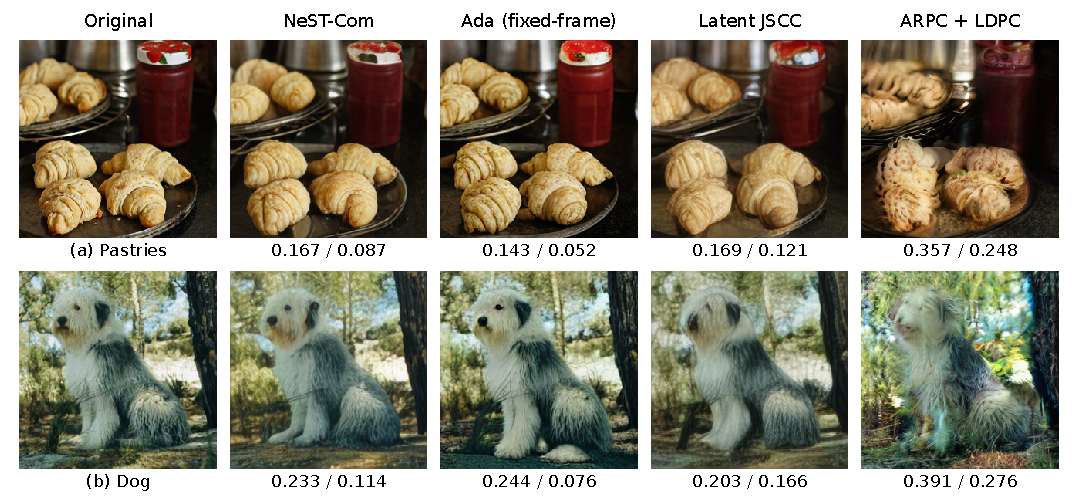
\includegraphics[width=\textwidth]{figure3.pdf}
\caption{Qualitative reconstructions of two development examples at $N=1024$ and 10~dB. Values denote LPIPS-Alex$\downarrow$ / DreamSim$\downarrow$. Ada denotes the fixed-frame adaptation.}
\label{fig:qualitative}
\end{figure*}
\fi
\begin{table}[t]
\caption{Pixel fidelity and image-feature similarity on common500 at $N=1024$. Each cell is PSNR (dB)$\uparrow$ / CLIP-I$\uparrow$. Ada denotes the fixed-frame adaptation. Values are source means.}
\label{tab:external}
\centering\footnotesize
\setlength{\tabcolsep}{3pt}
\begin{tabular}{lccc}
\toprule Method & 4 dB & 10 dB & 19 dB \\
\midrule
NeST-Com & 17.448 / 0.821 & 20.014 / 0.873 & 22.164 / 0.900 \\
Latent JSCC & 19.658 / 0.741 & 20.803 / 0.789 & 21.245 / 0.804 \\
SwinJSCC & 21.671 / 0.627 & 23.026 / 0.669 & 23.698 / 0.697 \\
BPG + LDPC & 20.743 / 0.586 & 22.543 / 0.635 & 24.230 / 0.684 \\
ARPC + LDPC & 14.184 / 0.644 & 16.471 / 0.713 & 18.199 / 0.788 \\
Ada (adapted) & 13.332 / 0.828 & 19.559 / 0.884 & 20.938 / 0.892 \\
\bottomrule
\end{tabular}
\end{table}

At all tested N1024 SNRs, NeST has lower mean LPIPS and DreamSim than the implemented SwinJSCC, BPG, and ARPC systems (Fig.~\ref{fig:performance}). Table~\ref{tab:external} shows the accompanying pixel-fidelity tradeoff: SwinJSCC and BPG have higher PSNR throughout. At 4~dB, Latent JSCC has higher PSNR and lower LPIPS than NeST, while NeST has lower DreamSim. These comparisons involve different tokenizers, priors, decoders, training, and conditioning.

Ada's relative performance depends on SNR and metric. At 10~dB it has better LPIPS, DreamSim, and CLIP-I; NeST has higher PSNR. Ada also has higher CLIP-I at 4~dB and slightly lower DreamSim at 19~dB. NeST exceeds Ada in PSNR by 4.116/0.455/1.226~dB at 4/10/19~dB. NeST, WHOLE, and Ada successfully reconstruct all 1500 evaluated transmissions per SNR, so overall and success-conditioned means coincide. The two development examples in Fig.~\ref{fig:qualitative} illustrate smoother pastry ridges and facial details with Latent JSCC and altered pastry shapes and dog pose with ARPC. NeST and Ada retain more of these structures but differ in detail; metric rankings vary by image.

\subsection{Transmission With a Reduced Symbol Budget}
\begin{table}[t]
\caption{Reduced-budget comparison on common500 at $N=512$. Differences are NeST-Com minus the fixed-frame Ada-TokenCom adaptation; brackets give source-paired 95\% CIs. Negative LPIPS and DreamSim favor NeST-Com.}
\label{tab:reduced}
\centering\footnotesize
\setlength{\tabcolsep}{4pt}
\begin{tabular}{ccc}
\toprule SNR & $\Delta$LPIPS & $\Delta$DreamSim \\
\midrule
4 & $-0.1890$ & $-0.1029$ \\
 & $[-0.1966,-0.1814]$ & $[-0.1142,-0.0917]$ \\
10 & $-0.1384$ & $-0.0660$ \\
 & $[-0.1440,-0.1328]$ & $[-0.0747,-0.0573]$ \\
19 & $-0.0245$ & $+0.0139$ \\
 & $[-0.0280,-0.0212]$ & $[0.0103,0.0173]$ \\
\bottomrule
\end{tabular}
\par\smallskip\begin{minipage}{\columnwidth}\footnotesize
Successful receptions (4/10/19~dB), each out of 1500: NeST 1496/1499/1500; WHOLE 1493/1500/1500; Ada 1495/1500/1500. All failures are body-CRC rejections retained as gray.
\end{minipage}
\end{table}

At $N=512$, NeST--WHOLE LPIPS differences are $-0.02995/-0.01548/-0.02749$ at 4/10/19~dB; DreamSim differences are $-0.04280/-0.01269/-0.02412$. All paired intervals favor NeST, as do PSNR (0.39--0.79~dB gains) and CLIP-I. At 10~dB both methods select target $(7,0)$ and 16-QAM rate 2/3. Both fall back for 99.6\% of sources, but NeST retains a within-scale prefix for 89.0\%. Mean retained tokens increase from 91.3 to 107.9 and source-bit utilization from 79.30\% to 93.46\%.

Against Ada, NeST has lower LPIPS at all three SNRs and lower DreamSim at 4/10~dB; Ada has lower DreamSim at 19~dB (Table~\ref{tab:reduced}) and higher CLIP-I throughout. WHOLE already exceeds Ada's mean PSNR by 3.79/3.66/0.95~dB; NeST increases these gaps to 4.180/4.055/1.740~dB. Joint-success comparisons retain all 500 sources and the same LPIPS/DreamSim directions; their PSNR gaps are 0.389/0.399/0.792~dB against WHOLE and 4.190/4.056/1.740~dB against Ada. These descriptive conditional results do not replace the failure-inclusive means (Supplement~S2.3).

On the fixed 100-image subset, replacing Ada's sampled tail by argmax leaves NeST higher in PSNR by 4.63/4.60~dB at $N=512$, 4/10~dB; the full perceptual sensitivity results are retained in Supplement~S3.